\begin{task}{32}
Приведите пример графа на 2015 вершинах, у которого ровно 1147 центральных вершин.
\end{task}
\begin{solution}
Требуемый граф состоит из клики на 1147 вершинах, к которым присоединены 868 вершин.

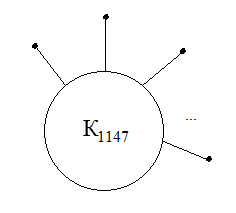
\includegraphics{img/id32.png}

Эксцентриситеты вершин клики равны 2, присоединенных вершин равны 3. Так как радиус графа равен 2, то все вершины клики являются центральными, а присоединенные ими не являются. Условие задачи выполнено.
\end{solution}